\documentclass{tufte-book}
%\documentclass[twoside,symmetric]{tufte-book}
\hypersetup{colorlinks}% uncomment this line if you prefer colored hyperlinks (e.g., for onscreen viewing)

%%
% Book metadata
<<<<<<< HEAD
\title{Introduction \\to Git\thanks{Thanks to Edward R.~Tufte for his inspiration.}}
\author[The Tufte-LaTeX Developers]{GermansEimer}
\publisher{The Invisible College}
=======
\title{Introduction \\to Python \thanks{Thanks to Edward R.~Tufte for his inspiration.}}
\author[The Tufte-LaTeX Developers]{CSEF}
\publisher{The Student Academy}
>>>>>>> upstream/master

%%
% If they're installed, use Bergamo and Chantilly from www.fontsite.com.
% They're clones of Bembo and Gill Sans, respectively.
%\IfFileExists{bergamo.sty}{\usepackage[osf]{bergamo}}{}% Bembo
%\IfFileExists{chantill.sty}{\usepackage{chantill}}{}% Gill Sans

%\usepackage{microtype}

%%
% Just some sample text
\usepackage{lipsum}

\usepackage{listings}
\renewcommand{\lstlistingname}{Listing}

%%
% For nicely typeset tabular material
\usepackage{booktabs}

%%
% For graphics / images
\usepackage{graphicx}
\setkeys{Gin}{width=\linewidth,totalheight=\textheight,keepaspectratio}
\graphicspath{{graphics/}}

%%
% Additional
\usepackage{units}
\usepackage{amsmath,amsfonts,amsthm} % Math packages
\usepackage{mathtools}% http://ctan.org/pkg/mathtools
%\usepackage{mparhack}
\usepackage{sectsty} % Allows customizing section commands
\usepackage[dvipsnames]{xcolor}
\usepackage{pgf,tikz}
\usepackage{pgfplots}
\usetikzlibrary{shapes,arrows}
\usetikzlibrary{patterns,fadings}
\usetikzlibrary{arrows}
 \usetikzlibrary{decorations.pathreplacing}
 \usetikzlibrary{snakes}
 \usetikzlibrary{spy}
 \usepackage{setspace}
% \usepackage{3dplot}
 \usepackage{cancel}
%\usepackage{physymb}
\usepackage{braket}
\usepackage{verbatim}
\usepackage{fancyvrb} % extended verbatim environments
\usepackage{framed}%To get shade behind text
\usepackage{pgfplots}
\usepackage{setspace}
\definecolor{shadecolor}{gray}{0.9}
%\usepackage[x11names]{xcolor}                     %Additional colors
%\usepackage{euler}  
\usepackage{framed}

%%%%%%%%%%%%%%%%%%%%%%%%%%%%%%%%%%%%%%%%%%%%%%%%%%%%%
% Default fixed font does not support bold face
\DeclareFixedFont{\ttb}{T1}{txtt}{bx}{n}{12} % for bold
\DeclareFixedFont{\ttm}{T1}{txtt}{m}{n}{12}  % for normal
% Custom colors
\usepackage{color}
\definecolor{normal}{rgb}{0,0.2,1}
\definecolor{lib}{rgb}{0.9,0.5,0}
\definecolor{str}{rgb}{0,0.7,0}
\definecolor{back}{rgb}{0.8,0.8,0.8}

\usepackage{listings}

% Python style for highlighting
\newcommand\pythonstyle{\lstset{
language=Python,
backgroundcolor=\color{back},
basicstyle=\ttm,
otherkeywords={*},             % Add keywords here
keywordstyle=\ttb\color{normal},
emph={__init__, in,from, import, and,not,or,as },          % Custom highlighting
emphstyle=\ttb\color{lib},    % Custom highlighting style
stringstyle=\color{str},
frame=single,
numbers=left,                         % Any extra options here
showstringspaces=false,
stepnumber=1,
commentstyle=\color{red}            % 
}}

% Python environment
\lstnewenvironment{python}[1][]
{
\pythonstyle
\lstset{#1}
}
{}

% Python for external files
\newcommand\pythonexternal[2][]{{
\pythonstyle
\lstinputlisting[#1]{#2}}}

% Python for inline
\newcommand\pythoninline[1]{{\pythonstyle\lstinline!#1!}}


%%%%%%%%%%%%%%%%%%%%%%%%%%%%%%%%%%%%%%%%%%%%%%%%%%%%%%%%%%


% The fancyvrb package lets us customize the formatting of verbatim
% environments.  We use a slightly smaller font.
\usepackage{fancyvrb}
\fvset{fontsize=\normalsize}

%%
% Prints argument within hanging parentheses (i.e., parentheses that take
% up no horizontal space).  Useful in tabular environments.
\newcommand{\hangp}[1]{\makebox[0pt][r]{(}#1\makebox[0pt][l]{)}}

%%
% Prints an asterisk that takes up no horizontal space.
% Useful in tabular environments.
\newcommand{\hangstar}{\makebox[0pt][l]{*}}

%%
% Prints a trailing space in a smart way.
\usepackage{xspace}




% Prints the month name (e.g., January) and the year (e.g., 2008)
\newcommand{\monthyear}{%
  \ifcase\month\or January\or February\or March\or April\or May\or June\or
  July\or August\or September\or October\or November\or
  December\fi\space\number\year
}


% Prints an epigraph and speaker in sans serif, all-caps type.
\newcommand{\openepigraph}[2]{%
  %\sffamily\fontsize{14}{16}\selectfont
  \begin{fullwidth}
  \sffamily\large
  \begin{doublespace}
  \noindent\allcaps{#1}\\% epigraph
  \noindent\allcaps{#2}% author
  \end{doublespace}
  \end{fullwidth}
}

% Inserts a blank page
\newcommand{\blankpage}{\newpage\hbox{}\thispagestyle{empty}\newpage}

\usepackage{units}

% Typesets the font size, leading, and measure in the form of 10/12x26 pc.
\newcommand{\measure}[3]{#1/#2$\times$\unit[#3]{pc}}

% Macros for typesetting the documentation
\newcommand{\hlred}[1]{\textcolor{Maroon}{#1}}% prints in red
\newcommand{\hangleft}[1]{\makebox[0pt][r]{#1}}
\newcommand{\hairsp}{\hspace{1pt}}% hair space
\newcommand{\hquad}{\hskip0.5em\relax}% half quad space
\newcommand{\TODO}{\textcolor{red}{\bf TODO!}\xspace}
\newcommand{\ie}{\textit{i.\hairsp{}e.}\xspace}
\newcommand{\eg}{\textit{e.\hairsp{}g.}\xspace}
\newcommand{\na}{\quad--}% used in tables for N/A cells
\providecommand{\XeLaTeX}{X\lower.5ex\hbox{\kern-0.15em\reflectbox{E}}\kern-0.1em\LaTeX}
\newcommand{\tXeLaTeX}{\XeLaTeX\index{XeLaTeX@\protect\XeLaTeX}}
% \index{\texttt{\textbackslash xyz}@\hangleft{\texttt{\textbackslash}}\texttt{xyz}}
\newcommand{\tuftebs}{\symbol{'134}}% a backslash in tt type in OT1/T1
\newcommand{\doccmdnoindex}[2][]{\texttt{\tuftebs#2}}% command name -- adds backslash automatically (and doesn't add cmd to the index)
\newcommand{\doccmddef}[2][]{%
  \hlred{\texttt{\tuftebs#2}}\label{cmd:#2}%
  \ifthenelse{\isempty{#1}}%
    {% add the command to the index
      \index{#2 command@\protect\hangleft{\texttt{\tuftebs}}\texttt{#2}}% command name
    }%
    {% add the command and package to the index
      \index{#2 command@\protect\hangleft{\texttt{\tuftebs}}\texttt{#2} (\texttt{#1} package)}% command name
      \index{#1 package@\texttt{#1} package}\index{packages!#1@\texttt{#1}}% package name
    }%
}% command name -- adds backslash automatically
\newcommand{\doccmd}[2][]{%
  \texttt{\tuftebs#2}%
  \ifthenelse{\isempty{#1}}%
    {% add the command to the index
      \index{#2 command@\protect\hangleft{\texttt{\tuftebs}}\texttt{#2}}% command name
    }%
    {% add the command and package to the index
      \index{#2 command@\protect\hangleft{\texttt{\tuftebs}}\texttt{#2} (\texttt{#1} package)}% command name
      \index{#1 package@\texttt{#1} package}\index{packages!#1@\texttt{#1}}% package name
    }%
}% command name -- adds backslash automatically
\newcommand{\docopt}[1]{\ensuremath{\langle}\textrm{\textit{#1}}\ensuremath{\rangle}}% optional command argument
\newcommand{\docarg}[1]{\textrm{\textit{#1}}}% (required) command argument
\newenvironment{docspec}{\begin{quotation}\ttfamily\parskip0pt\parindent0pt\ignorespaces}{\end{quotation}}% command specification environment
\newcommand{\docenv}[1]{\texttt{#1}\index{#1 environment@\texttt{#1} environment}\index{environments!#1@\texttt{#1}}}% environment name
\newcommand{\docenvdef}[1]{\hlred{\texttt{#1}}\label{env:#1}\index{#1 environment@\texttt{#1} environment}\index{environments!#1@\texttt{#1}}}% environment name
\newcommand{\docpkg}[1]{\texttt{#1}\index{#1 package@\texttt{#1} package}\index{packages!#1@\texttt{#1}}}% package name
\newcommand{\doccls}[1]{\texttt{#1}}% document class name
\newcommand{\docclsopt}[1]{\texttt{#1}\index{#1 class option@\texttt{#1} class option}\index{class options!#1@\texttt{#1}}}% document class option name
\newcommand{\docclsoptdef}[1]{\hlred{\texttt{#1}}\label{clsopt:#1}\index{#1 class option@\texttt{#1} class option}\index{class options!#1@\texttt{#1}}}% document class option name defined
\newcommand{\docmsg}[2]{\bigskip\begin{fullwidth}\noindent\ttfamily#1\end{fullwidth}\medskip\par\noindent#2}
\newcommand{\docfilehook}[2]{\texttt{#1}\index{file hooks!#2}\index{#1@\texttt{#1}}}
\newcommand{\doccounter}[1]{\texttt{#1}\index{#1 counter@\texttt{#1} counter}}

% Generates the index
\usepackage{makeidx}
\makeindex

\begin{document}

% Front matter
\frontmatter

% r.1 blank page
%\blankpage

% v.2 epigraphs
\newpage\thispagestyle{empty}

\openepigraph{%
The only shibboleth the West has is science. It is the premise of modernity and it defines itself as a rationality capable of, indeed requiring separation from politics, religion and really, society. Modernisation is to work towards this.
}{Bruno Latour}
\vfill
\openepigraph{%
The boundary between science fiction and social reality is an optical illusion.
}{Donna Haraway}


% r.3 full title page
\maketitle




% r.5 contents
\tableofcontents

\listoffigures

\listoftables

% r.7 dedication
\cleardoublepage
~\vfill
\begin{doublespace}
\noindent\fontsize{18}{22}\selectfont\itshape
\nohyphenation
The longest snake ever held captive is Medusa, a reticulated python (python reticulatus). On 12 October 2011, she was measured at 7.67 m long.% \mbox{Edward R.~Tufte} 
%and \mbox{Donald E.~Knuth}.
\end{doublespace}
\vfill
\vfill


% r.9 introduction
%\cleardoublepage
\chapter*{Note}

This physics text is an OpenSource academic project developed in abstraction at The Academy.  The manuscript is written in \LaTeX \ and makes use of the \doccls{tufte-book} and \doccls{tufte-handout} document classes.  

\vspace{2cm}

http://latex-project.org/ftp.html

https://git-scm.com/downloads

%%
% Start the main matter (normal chapters)
\mainmatter

<<<<<<< HEAD

Introduction to OSX Terminal

Terminal (Terminal.app) is the terminal emulator included in the OS X operating system by Apple. (Wikipedia)

A terminal emulator is an application that allows access to the operating system. This emulator can be used to perform multiple tasks; it can perform from simple tasks like printing out text, to performing more complex tasks like uploading files to the cloud.


%\include{translational_kinematics}

%\include{introduction}


%\section{\textbf{For Loops, Nested For Loops}}
For in loop has the ability to iterate over the items of any sequence, such as a list or a string.

If a sequence contains an expression list, it is evaluated first. Then, the first item in the sequence is assigned to the iterating variable iterating var. Next, the statements block is executed. Each item in the list is assigned to iterating var, and the statement(s) block is executed until the entire sequence is exhausted.
\end{abstract}

\normalsize

\section{\textbf{PYTHON CODE}}

\section{\textbf{Syntax:}}
\begin{verbatim}
for var in sequence:
   statements
\end{verbatim}
   
\section{\textbf{example #1:}}   
\marginnote[40pt]{The goal is to print all the elements in the array}
\begin{shaded}
\begin{verbatim}
for i in ["hello", "hey", "yo"]:
    print i
\end{verbatim}
\end{shaded}

\section{\textbf{Output #1:}}
\begin{shaded}
\begin{verbatim}
>>> Hello
    hey
    yo
\end{verbatim}
\end{shaded}

\section{\textbf{example #2:}}   
\marginnote[40pt]{The goal is to print all the number in range 5. Note, that Python starts counting from 0}
\begin{shaded}
\begin{verbatim}
for i in range(5):
    print i
\end{verbatim}
\end{shaded}
    
\section{\textbf{Output #2:}}
\begin{shaded}
\begin{verbatim}
>>> 1
    2
    3
    4
    5
\end{verbatim}
\end{shaded}

\vspace{2cm}

\section{\textbf{NESTED FOR LOOPS}}
\begin{verbatim}
Python programming language allows to use one loop inside 
another loop. Following section shows few examples to illustrate
the concept.
\end{verbatim}


\section{\textbf{Syntax:}}
\begin{verbatim}
for iterating_var in sequence:
   for iterating_var in sequence:
      statements(s)
   statements(s)
\end{verbatim}

\section{\textbf{example #1:}}   
\marginnote[40pt]{The goal is to print every number from 0 to 5 three times in a row.}
\begin{shaded}
\begin{verbatim}
for i in range(5): #loop everything indented 5 times
    for j in range(3): #loop everything indented 3 times
        print i #print output of i

\end{verbatim}
\end{shaded}

\vspace{3cm}
\section{\textbf{Output 1:}}
\begin{shaded}
\begin{verbatim}
>>> 0
    0
    0
    1
    1
    1
    2
    2
    2
    3
    3
    3
    4
    4
    4
\end{verbatim}
\end{shaded}

\vspace{1cm}

\section{\textbf{example #2:}}   
\marginnote[40pt]{The goal is to create a 2D arrays that would be fulfilled with values of "1" or "0" depending on which number was randomly chosen by the computer}

\scriptsize
\begin{shaded}
\begin{verbatim}

import random #importing "random" library that will take random numbers for our program
x = [] #creating initial, empty array that will be fulfilled with other arrays later
for i in range(5): #loop everything indented 5 times
    r=[] #creates 5 more arrays
    for j in range(5): #loop everything indented 5 times
        if random.uniform(0,10)<3: #compare if randomly chosen number is smaller than 3
            r=r+[1] #if it is, add value of "1" inside the secondary array - r
        else: #or
            r=r+[0] #if it is bigger, add value of "0" inside the secondary array - r
    x.append(r) #add all of these secondary arrays to our main - x array. 
    #Basically we create 2D array.
print x #print our 2D array to see the output.

\end{verbatim}
\end{shaded}

\normalsize
\section{\textbf{Output 2:}}
\marginnote[40pt]{However, the numbers that you see here isn't the only output you can get. We used random uniforms and each time it will give different values.}
\begin{shaded}
\begin{verbatim}
>>> [[0, 0, 0, 1, 1], [1, 0, 0, 0, 0], [0, 0, 0, 0, 0],
    [0, 1, 0, 0, 0], [0, 0, 0, 0, 0]]
\end{verbatim}
\end{shaded}
   



%ints and floats
%\chapter{Boolean}

\section{Intro}

boolean boolean

\section{Boolean Operators}

\section{Boolean Arithmetic}

\chapter{Array 1-D, 2-D, 3-D}
\section{Intro}
	Array is like a storage, it can fill with string or integer. In 1-D, 2-D it can also represents the x-axis and y axis.
\section{Creating arrays}
	Arrays is created buy blanket.\\ \ \\
\noindent Example:\\
\begin{verbatim}
	a=[ ]        *a is the array name that you want.
\end{verbatim}
The things in the [ ] and be store and when you want to access it you will need its position in the array and type like  a[0]\\ \ \\
\noindent Example:\\
\begin{verbatim}
	a=["apple","orange","banana"]
\end{verbatim}
If you want to print banana form the array, you may want to type\\
\begin{verbatim}
print a[2] 
\end{verbatim}
\section{Filling arrays}
	Everything can be store in the array, strings, integers, arrays. When you create an array you can fill things in it as the default  things that the array have.\\ \ \\
\noindent Example:
\begin{verbatim}
    a=["Billy","Bud",90,60,50]
    b=["Anne","Chow",90,95,100]
    c=["Jen","Bo",60,80,90]
\end{verbatim}

If you want to add things into the array that u create already, you can use \\ \ \\

\begin{verbatim}
     array_name=array_name+[Things you want to add]
\end{verbatim}

\noindent Example:\\ \ \\

\begin{verbatim}	
    a=[apple]
\end{verbatim}

\noindent and now I want to add orange into it, so we add\\ \ \\

\begin{verbatim}
    a=a+[orange]
\end{verbatim}	

\noindent To create 2-D or more array we need to create array in the nested for-loop.\\ \ \\
\noindent Example:
\begin{verbatim}
a=[]
for i in range(N):	*N how long you want the array to be
    b=[]    *This is a temporary array to generate every array inside the main array.
    for j in range(N):
        *Things you want to put in the array by b=b+[ ]
    a=a+[b]	    *Here put the temporary array back to the main array.
\end{verbatim}		


\section{Traversing array}
Traversing array is visiting each element in the array and do something. In 1-D we can do it with for loop to identify things in array.
Example:

\begin{verbatim}
a=[1,2,3]
for i in range(len(a))    *len(a) =  Numbers of elements in the array
    *Things put here can edit the specific element a[i]
\end{verbatim}
	
\noindent In 2-D we start using nested for-loop to identify the x-axis and y-axis. So we use nested for-loop to traversing it too.\\ \ \\
\noindent Example:
\begin{verbatim}
a=[[0,1],[0,0],[0,1]]
for i in range(len(a)):
    for j in range(len(a)):
        *Things put here can edit the specific element a[i][j]
\end{verbatim}
			
\noindent In 3-D we use more for-loop to identify the more dimension.\\ \ \\
\noindent Example:
\begin{verbatim}
a=[[[0,0],[0,0]],[[0,0],[0,0]]]
for x in range(len(a)):
    for y in range(len(a)):
        for z in range(len(a)):
            *Things put here can edit the specific element a[x][y][z]
\end{verbatim}
	
	
	
	
	
	

=======
\chapter{Integers and Floating Point Numbers}

\section{What is Integer?}
An integer (from the Latin integer meaning "whole") [note 1] is a number that can be written without a fractional component. For example, 21, 4, 0, and −2048 are integers, while 9.75, 5½, and √2 are not.

\begin{figure}[h!]
\centering

\includegraphics[scale=1.7]{universe.jpg}
\caption{The ultimate answer of the universe is also an Integer!}
\citep{adams1995hitchhiker}
\label{fig:univerise}
\end{figure}

\section{Floating point!}
Also called floats, they represent real numbers and are written with a decimal point dividing the integer and fractional parts. 
You can convert an integer to a floating number by your python and vice versa! :

\begin{verbatim}
Type int(x) to convert x to a plain integer.
                                                                                                            
Type: int(4.22222)
Result: 4


Type float(x) to convert x to a floating-point number.

type: float(1)
Result: 1.0
\end{verbatim}



\section{Number Type Conversion}
Python converts numbers internally in an expression containing mixed types to a common type for evaluation. But sometimes, you need to coerce a number explicitly from one type to another to satisfy the requirements of an operator or function parameter.




\section{\textbf{Definition:}}

Booleans:

In Python we have the following terms (characters and phrases) for determining if something is "True" or "False." Logic on a computer is all about seeing if some combination of these characters and some variables is True at that point in the program.

and


or


not


!= (not equal)


== (equal)


>= (greater-than-equal)


<= (less-than-equal)


True


False


We use these characters to make the truth or not.


NOT:


not False =	True


not True = False


OR:


True or False = True


True or True = True


False or True = True


False or False = False

AND:


True and False = False


True and True = True


False and True = False


False and False = False


NOT OR:


not (True or False) = False


not (True or True) = False


not (False or True) = False


not (False or False) = True


NOT AND:


not (True and False) = True


not (True and True)	= False


not (False and True) = True


not (False and False) =	True


!=:


1 != 0 = True


1 != 1 = False


0 != 1 = True


0 != 0 = False



==:


1 == 0 = False


1 == 1 = True


0 == 1 = False


0 == 0 = True
\definecolor{shadecolor}{rgb}{0.9,0.9,0.9}











\chapter{While Loops}

A {\color{red}while loop} statement in Python programming language repeatedly executes a target statement as long as a given condition is true.

\vspace{1cm}
The condition may be any expression, and true is any non-zero value. The loop iterates while the condition is true.When the condition becomes false, program control passes to the line immediately following the loop.In Python, all the statements indented by the same number of character spaces after a programming construct are considered to be part of a single block of code. Python uses indentation as its method of grouping statements.

\begin{marginfigure}
  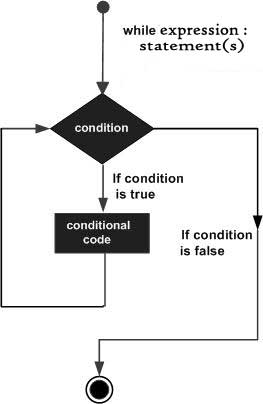
\includegraphics[width=\linewidth]{whileloop.jpeg}
  \caption{Flow diagram about how the while loop works}
  \label{fig:marginfig}
\end{marginfigure}

\vspace{0.5cm}
\subsection{Python code example}
\begin{framed}
\begin{verbatim}

count = 0
while (count < 9):
   print 'The count is:', count
   count = count + 1

print "Good bye!"

\end{verbatim}
\end{framed}

\subsection{Output}
\marginnote[40pt]{The code will produce the following output.}
\begin{shaded}
\begin{verbatim}
>>> 
The count is: 0
The count is: 1
The count is: 2
The count is: 3
The count is: 4
The count is: 5
The count is: 6
The count is: 7
The count is: 8
Good bye!
>>> 
\end{verbatim}
\end{shaded}

\subsection{Infinite Loop}
A loop becomes {\color{red}infinite loop} if a condition never becomes {\textbf{FALSE}}. You must use caution when using while loops because of the possibility that this condition never resolves to a FALSE value. This results in a loop that never ends. Such a loop is called an infinite loop.

An infinite loop might be useful in client/server programming where the server needs to run continuously so that client programs can communicate with it as and when required.
\marginnote[40pt]{This python code is an example of how infinite loop can be created.}
\begin{framed}
\begin{verbatim}
var = 1
while var == 1:
   num = raw_input("Enter a number  :")
   print "You entered: ", num

print "Good bye!"
\end{verbatim}
\end{framed}

\marginnote[40pt]{This code creates an infinite loop where it will need your input of any number.Once you input any number, it will output it like if you input "X" it will show back "X".}
\begin{shaded}
\begin{verbatim}

Enter a number  :X
You entered:  x
Enter a number  :Y
You entered:  Y
Enter a number  :Z
You entered:  Z
Enter a number between :

\end{verbatim}
\end{shaded}

To break the loop you will either need to add the "{\color{red}break}" command in your code OR press {\textbf{CTRL+C} to exit the program.

\subsection{Using else statements with while loops}
Python supports to have an else statement associated with a loop statement.

If the {\color{red}else statement} is used with a while loop, the else statement is executed when the condition becomes false.

\vspace{1cm}







\begin{framed}
\begin{verbatim}

count = 0
while count < 5:
   print count, " is  less than 5"
   count = count + 1
else:
   print count, " is not less than 5"

\end{verbatim}
\end{framed}

\marginnote[-140pt]{The following code illustrates the combination of an else statement with a while statement that prints a number as long as it is less than 5, otherwise else statement gets executed.}

\marginnote[40pt]{This is the output in python when the code above is executed.}
\begin{shaded}
\begin{verbatim}
>>> 
0 is less than 5
1 is less than 5
2 is less than 5
3 is less than 5
4 is less than 5
5 is not less than 5
>>> 
\end{verbatim}
\end{shaded}






\chapter{While Loops}
A while loop is a function, which needs a boolean statement to run, in order to prit out a list of results. The while loop will print out as many resultts as possible, until the boolean statement stops being true. For example:

\begin{verbatim}
i=0
while (i<5):
    print i
    i=i+1
    
\end{verbatim}

Now, the boolean statement inserted here is "i<5", meaning that "i" must be less than 5. The next function now commands the system to print "i". The result would be:
\begin{verbatim}
0
1
2
3
4
\end{verbatim}

This is because after the computer was demanded to print out "i", the function "i==i+1", was entered, meaning that it should print out all the numbers that make the bolean statement rue, until the number is five, making it false.

There are also many ways you could manipulate this code. A break may be inserted as follows: 
\begin{verbatim}
i=0
while (i<5):
    print i
    i=i+
    if i==4:
        break
    
\end{verbatim}

The result would be:
\begin{verbatim}
0
1
2
3
\end{verbatim}

Excluding "4", because as a result of the break, the computer is now told not to print anything from the number 4.

However, if the break came before "i=i+1" like:
\begin{verbatim}
i=0
while (i<5):
    print i
    if i==4:
        break
    i=i+1
    
\end{verbatim}

The result would be:
\begin{verbatim}
0
1
2
3
4
\end{verbatim}













\chapter{Bases}
The word "base" in mathematics is used to refer to a particular mathematical object that is used as a building block. The most common uses are the related concepts of the number system whose digits are used to represent numbers. In common, people use decimal system. However, the computers are compsed with binary system. Also, SHA-256 gives the hexadecimal code.
\section{Binary}
Binary is composed with only 0 and 1. Each of digits represents 2 to the power of something. From the right to left, it starts from $2^0$ to increasing the power.
	
\section{Decimals}
Decimal system is what people use in usual days. It is composed with 0,1,2,3,4,5,6,7,8, and 9, and it starts from $10^0$ and increases the power of 10 when it goes the next digit. The reason why people use the decimal system is that the human has 10 fingers, so the calculation is easier and more simple. 
\section{Hexadecimals}
Hexadecimal system is used for computer languages such as C language/C++ and SHA-256.It is composed with 1,2,3,4,5,6,7,8,9,a,b,c,d,e, and f. When the decimal numbers are hashed by SHA-256, it is more difficult if hashed number starts with 0 and have many 0s in the number. The number in front of x is the number of 0s which is leading.
\section{Conversion}
\begin{figure}
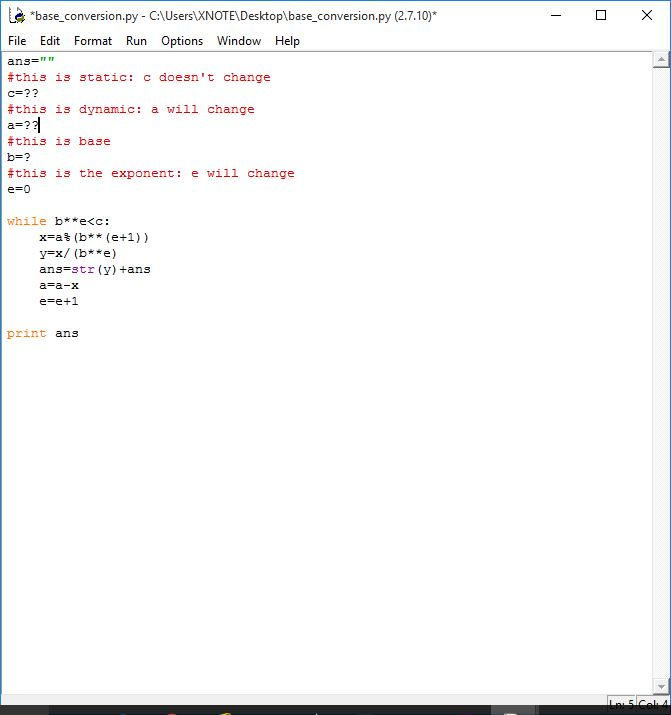
\includegraphics[width=10cm]{BaseConversion.jpg}
\end{figure}
It is the sample code of the base conversion. ? is what the base is, so it can be any decimal number. ?? can also be the any number, but decimal numbers. It changes from decimal numbers to base of ? numbers. a needs to be subtracted by x for the next step getting ? to the power of next exponent. Then, repeat the previous steps with e added 1. And then, repeat for next step again. At the last, however, y whicch is the quotient of the last x divided b to the power of e should be concantenated with ans. The quotient becomes the first number of the ? base numbers.

\chapter{Array 1-D, 2-D, 3-D}
\section{Intro}
	Array is like a storage, it can fill with string or integer. In 1-D, 2-D it can also represents the x-axis and y axis.
\section{Creating arrays}
	Arrays is created buy blanket.\\ \ \\
\noindent Example:\\
\begin{verbatim}
	a=[ ]        *a is the array name that you want.
\end{verbatim}
The things in the [ ] and be store and when you want to access it you will need its position in the array and type like  a[0]\\ \ \\
\noindent Example:\\
\begin{verbatim}
	a=["apple","orange","banana"]
\end{verbatim}
If you want to print banana form the array, you may want to type\\
\begin{verbatim}
print a[2] 
\end{verbatim}
\section{Filling arrays}
	Everything can be store in the array, strings, integers, arrays. When you create an array you can fill things in it as the default  things that the array have.\\ \ \\
\noindent Example:
\begin{verbatim}
    a=["Billy","Bud",90,60,50]
    b=["Anne","Chow",90,95,100]
    c=["Jen","Bo",60,80,90]
\end{verbatim}

If you want to add things into the array that u create already, you can use \\ \ \\

\begin{verbatim}
     array_name=array_name+[Things you want to add]
\end{verbatim}

\noindent Example:\\ \ \\

\begin{verbatim}	
    a=[apple]
\end{verbatim}

\noindent and now I want to add orange into it, so we add\\ \ \\

\begin{verbatim}
    a=a+[orange]
\end{verbatim}	

\noindent To create 2-D or more array we need to create array in the nested for-loop.\\ \ \\
\noindent Example:
\begin{verbatim}
a=[]
for i in range(N):	*N how long you want the array to be
    b=[]    *This is a temporary array to generate every array inside the main array.
    for j in range(N):
        *Things you want to put in the array by b=b+[ ]
    a=a+[b]	    *Here put the temporary array back to the main array.
\end{verbatim}		


\section{Traversing array}
Traversing array is visiting each element in the array and do something. In 1-D we can do it with for loop to identify things in array.
Example:

\begin{verbatim}
a=[1,2,3]
for i in range(len(a))    *len(a) =  Numbers of elements in the array
    *Things put here can edit the specific element a[i]
\end{verbatim}
	
\noindent In 2-D we start using nested for-loop to identify the x-axis and y-axis. So we use nested for-loop to traversing it too.\\ \ \\
\noindent Example:
\begin{verbatim}
a=[[0,1],[0,0],[0,1]]
for i in range(len(a)):
    for j in range(len(a)):
        *Things put here can edit the specific element a[i][j]
\end{verbatim}
			
\noindent In 3-D we use more for-loop to identify the more dimension.\\ \ \\
\noindent Example:
\begin{verbatim}
a=[[[0,0],[0,0]],[[0,0],[0,0]]]
for x in range(len(a)):
    for y in range(len(a)):
        for z in range(len(a)):
            *Things put here can edit the specific element a[x][y][z]
\end{verbatim}
	
	
	
	
	
	






\chapter{Arrays}

In a nutshell, arrays are lists of data. Most commonly, they are sets
of integers, although they can also be sets of strings. There are
many uses for an array, such as being used as a database to count
occurrences. The simplest arrays are one-dimensional arrays, which
look like this.

\begin{lstlisting}
[0,1,2,3,4]
["a","b","c","d","e"]
\end{lstlisting}


These arrays can be described with several different characteristics.
\begin{enumerate}
\item They are both an array of length 5.
\item They are both one dimensional arrays (trust me, this will make more
sense).
\item The first is a list of integers, and the second is a list of strings.
\end{enumerate}

\subparagraph{Array generation}

Arrays are generated in a program by first creating an empty array,
or by creating an array that is already filled with whatever you'd
like.

\begin{lstlisting}
a = []
savoryfillings = ["meat","cheese","potato"]
\end{lstlisting}



\subparagraph{Adding to an array}

Adding to an array, also known as ``concatenation'', is also a very
simple process, much like generating an array. A simple way to fill
an array with, let's say, zeroes, is with a for loop.

\begin{lstlisting}
a = []
for i in range(5):
	a = a + [0]
print a
#this program will yield [0, 0, 0, 0, 0]
\end{lstlisting}


Note how the zero is in brackets. This will signify to the interpreter
that this zero is intended to be a unit of the array.

Strings can also be concatenated to an array of strings.

\begin{lstlisting}
>>> savoryfillings = ["meat","cheese","potato"] 
>>> savoryfillings = savoryfillings + ["spinach"] 
>>> print savoryfillings 
['meat', 'cheese', 'potato', 'spinach']
\end{lstlisting}



\subparagraph{Referencing certain parts of an array}

Referencing certain parts of an array is rather simple. A simple program
that does such thing and prints the referenced points is displayed
below. Remember that Python starts counting at 0, not 1!

\begin{lstlisting}
>>> a = [1, 2, 3, 4]
>>> x = a[0]
>>> y = a[1]
>>> #referencing points of array is done by (nameofarray)[pointinarray]
>>> print x
>>> print y
1
2
\end{lstlisting}



\subparagraph{The command 'len'}

The 'len' command takes the length of a given array and converts it
into an integer. 

\begin{lstlisting}
>>> a = [1, 2, 3]
>>> x = len(a)
>>> print x
3
\end{lstlisting}


'len' can also be used to do something to every point of an array,
with the use of a for loop.

\begin{lstlisting}
>>> a = [0, 1, 2, 3, 4, 5]
>>> for i in range(len(a)): 	
	a[i] = a[i] + 1

>>> print a 
[1, 2, 3, 4, 5, 6]  
\end{lstlisting}



\subparagraph{Two-/three-dimensional arrays}

Multidimensional arrays can be created through the use of nested for
loops - for example, the program below generates a 5x5 array of zeroes.

\begin{lstlisting}
>>> a = [] 
>>> for i in range(5):     
		b = []     
		for j in range(5):         
			b = b+[0]     
		a = a+[b] 
>>> print a
[[0, 0, 0, 0, 0], [0, 0, 0, 0, 0], [0, 0, 0, 0, 0], [0, 0, 0, 0, 0], [0, 0, 0, 0, 0]]
\end{lstlisting}


Note how this two-dimensional array has five arrays within it, each
with five zeroes.


\subparagraph{Application of arrays}

Arrays can be used to catalog data. This program logs 

\begin{lstlisting}
import random
mastercount = []
for i in range (10):
	mastercount = mastercount + [0]
for i in range (1000):
	x = random.randint(0,9)
	mastercount[x] = mastercount[x]+1
print mastercount
#sample yield of program - [95, 103, 96, 98, 107, 108, 101, 107, 102, 83]
\end{lstlisting}


\section{\textbf{For Loops, Nested For Loops}}
For in loop has the ability to iterate over the items of any sequence, such as a list or a string.

If a sequence contains an expression list, it is evaluated first. Then, the first item in the sequence is assigned to the iterating variable iterating var. Next, the statements block is executed. Each item in the list is assigned to iterating var, and the statement(s) block is executed until the entire sequence is exhausted.
\end{abstract}

\normalsize

\section{\textbf{PYTHON CODE}}

\section{\textbf{Syntax:}}
\begin{verbatim}
for var in sequence:
   statements
\end{verbatim}
   
\section{\textbf{example #1:}}   
\marginnote[40pt]{The goal is to print all the elements in the array}
\begin{shaded}
\begin{verbatim}
for i in ["hello", "hey", "yo"]:
    print i
\end{verbatim}
\end{shaded}

\section{\textbf{Output #1:}}
\begin{shaded}
\begin{verbatim}
>>> Hello
    hey
    yo
\end{verbatim}
\end{shaded}

\section{\textbf{example #2:}}   
\marginnote[40pt]{The goal is to print all the number in range 5. Note, that Python starts counting from 0}
\begin{shaded}
\begin{verbatim}
for i in range(5):
    print i
\end{verbatim}
\end{shaded}
    
\section{\textbf{Output #2:}}
\begin{shaded}
\begin{verbatim}
>>> 1
    2
    3
    4
    5
\end{verbatim}
\end{shaded}

\vspace{2cm}

\section{\textbf{NESTED FOR LOOPS}}
\begin{verbatim}
Python programming language allows to use one loop inside 
another loop. Following section shows few examples to illustrate
the concept.
\end{verbatim}


\section{\textbf{Syntax:}}
\begin{verbatim}
for iterating_var in sequence:
   for iterating_var in sequence:
      statements(s)
   statements(s)
\end{verbatim}

\section{\textbf{example #1:}}   
\marginnote[40pt]{The goal is to print every number from 0 to 5 three times in a row.}
\begin{shaded}
\begin{verbatim}
for i in range(5): #loop everything indented 5 times
    for j in range(3): #loop everything indented 3 times
        print i #print output of i

\end{verbatim}
\end{shaded}

\vspace{3cm}
\section{\textbf{Output 1:}}
\begin{shaded}
\begin{verbatim}
>>> 0
    0
    0
    1
    1
    1
    2
    2
    2
    3
    3
    3
    4
    4
    4
\end{verbatim}
\end{shaded}

\vspace{1cm}

\section{\textbf{example #2:}}   
\marginnote[40pt]{The goal is to create a 2D arrays that would be fulfilled with values of "1" or "0" depending on which number was randomly chosen by the computer}

\scriptsize
\begin{shaded}
\begin{verbatim}

import random #importing "random" library that will take random numbers for our program
x = [] #creating initial, empty array that will be fulfilled with other arrays later
for i in range(5): #loop everything indented 5 times
    r=[] #creates 5 more arrays
    for j in range(5): #loop everything indented 5 times
        if random.uniform(0,10)<3: #compare if randomly chosen number is smaller than 3
            r=r+[1] #if it is, add value of "1" inside the secondary array - r
        else: #or
            r=r+[0] #if it is bigger, add value of "0" inside the secondary array - r
    x.append(r) #add all of these secondary arrays to our main - x array. 
    #Basically we create 2D array.
print x #print our 2D array to see the output.

\end{verbatim}
\end{shaded}

\normalsize
\section{\textbf{Output 2:}}
\marginnote[40pt]{However, the numbers that you see here isn't the only output you can get. We used random uniforms and each time it will give different values.}
\begin{shaded}
\begin{verbatim}
>>> [[0, 0, 0, 1, 1], [1, 0, 0, 0, 0], [0, 0, 0, 0, 0],
    [0, 1, 0, 0, 0], [0, 0, 0, 0, 0]]
\end{verbatim}
\end{shaded}
   
\include{libraries_intro}
\chapter{Random}
\section{Intro}
Random is a library that you can used to generate random numbers in python.
\section{Creating random numbers}
You can use a code to generate random numbers.
\begin{verbatim}
import random    *You need to import random before you generate random numbers
random.uniform(minimum,maximum)
\end{verbatim}
while minimum and maximum number can be intergers(0) or floats(0.0)

\section{Usage of random number}
Simply here is a example of how to add random numbers to an array
\begin{verbatim}
import random
a=[]
for i in range(N):    *N is the the number of how many random numbers you want to add to the array
    a=a+[random.uniform(0,100)]   
         *0 is the minimum number and 100 is the maximum number, they are variable, you can change to 
          numbers you want.
    
\end{verbatim}
Here is a example of using random function to randomly fill a 2-D array with 0 and 1 by how many percentage you want it is filled.

\begin{verbatim}
import random
def fill(a,p):    *a is the name or you 2-D array    *p is the percentage you want, such as: 0.1, 0.25....
    for i in range(len(a)):    *len(a) is the length of you array
        for j in range(len(a)):
        	    if random.uniform(0,1)<p:
	        a[i][j]=1
	    else:
	        a[i][j]=0
\end{verbatim}

\chapter{Statistics Library}

\section{Introduction}
This statistics library includes eight functions that we can use to deal with a set of data. \\
\textit{Tips}
\begin{itemize}
\item \textit{Additional libraries are needed}
\item \textit{Multiple functions are needed for some operations}
\end{itemize}

\section{Zero}

\begin{equation}
\centering
$$\begin{verbatim}
def zeros(n):
    a=[]
    for i in range(n):
        a=a+[0]
    return a
\end{verbatim}
$$\end{equation}
This function can be used to create a consecutive and repeating array(all elements are the same). \\
\noindent \textit{Example:}
\begin{verbatim}
def zero(n):
    a=[]
    for i in range(n):
        a=a+[0]
    return a

print zero(9)
\end{verbatim} 
\textit{Output:} 
\texttt{ [0, 0, 0, 0, 0, 0, 0, 0, 0] }

\section{Summing an array}
\begin{equation}
$$\begin{verbatim}
def sum_array(a):
    s=0
    for i in range(len(a)):
        s=s+a[i]
    return s
\end{verbatim}
$$\end{equation}
This function can help us to sum up all the elements in an array. \\
\noindent \textit{Example:} 
\begin{verbatim}
a=[1,2,3,4]
def sum_array(a):
    s=0
    for i in range(len(a)):
        s=s+a[i]
    return s
print sum_array(a)
\end{verbatim} 
\textit{Output:}
\texttt{10}

\section{Finding means}
\begin{equation}
$$\begin{verbatim}
def avg(a):
    return sum_array(a)/len(a)
\end{verbatim}
$$\end{equation}
This function can help us to calculate the mean of all the data in an array, and we need assistance of the sum function. \\
\noindent \textit{Example:} 
\begin{verbatim}
a=[23,19,25,21]
def sum_array(a):
    s=0
    for i in range(len(a)):
        s=s+a[i]
    return s

def avg(a):
    return sum_array(a)/len(a)

print avg(a)
\end{verbatim} 
\textit{Output:}
\texttt{22}

\section{Variance}
\begin{equation}
$$\begin{verbatim}
def var(a):
    s=0
    for i in range(len(a)):
        s=s+a[i]**2
    m=avg(a)
    return (s/len(a)-m**2)
\end{verbatim}
$$\end{equation}
This function can help us to find the variance of the data.Also, we need the assistance of the average function. \\
\noindent \textit{Example:}
\begin{verbatim}
a=[23,19,25,21]
def sum_array(a):
    s=0
    for i in range(len(a)):
        s=s+a[i]
    return s

def avg(a):
    return sum_array(a)/len(a)

print avg(a)

def var(a):
    s=0
    for i in range(len(a)):
        s=s+a[i]**2
    m=avg(a)
    return (s/len(a)-m**2)
print var(a)
\end{verbatim}
\textit{Output: 5}

\section{Construct an array of random numbers}
\begin{equation}
$$\begin{verbatim}
def rand_array(n,mini,maxi):
    a=[]
    for i in range(n):
        a=a+[random.uniform(mini,maxi)]
    return a
\end{verbatim}
$$\end{equation}
We can use this function to construct an array filled with random numbers. We need the random library to run the function.Here n represents the number of elements in the array; mini is the minimum value of the elements;maxi is the maximum value

\section{To fill a histogram} \textit{Library "graphics" is needed*}
\begin{equation}
$$\begin{verbatim}
def histogram(mini,maxi,bins,a):
    h=zeros(bins)
    w=(maxi-mini)/bins
    for i in range(len(a)):
        for j in range(bins):
            if (a[i]>(mini+j*w))and a[i]<(mini+(j+1)*w):
                h[j]=h[j]+1
    return h
\end{verbatim}
$$\end{equation}
The four arguments in parenthesis are decisive for the histogram.
Here mini represents the minimum value in the data;
maxi represents the maximum value in the data;
bin represents the number of different groups of data;
a is the number of all the data.

\section{Find the maximum value}
\begin{equation}
$$\begin{verbatim}
def maximum(a):
    m=0
    for i in range(len(a)):
        if a[i]>m:
            m=a[i]
    return m
\end{verbatim}
$$\end{equation}
This funciton can help us to identify the maximum value in the data.

\section{Drawing a histogram} \textit{Library "graphics" is needed}\\
\noindent To draw a histogram, we first need to define a function that can draw a bargragh:
\begin{equation}
$$\begin{verbatim}
def bar(a,win):
    win.setCoords(-1,-1,len(a)+1,maximum(a)+1)
    bl=[]
    tr=[]
    rec=[]
    for i in range(len(a)):
        bl=bl+[Point(i,0)]
        tr=tr+[Point(i+a,a[i])]
        rec=rec+[Rectangle(bl[i],tr[i])]
        rec[i].draw(win)
\end{verbatim}
$$\end{equation} \\
Then we combine the "bar" function and the "histogram" function.\\
\noindent \textit{Here is just an example:}
\begin{equation}
$$\begin{verbatim}
def main():
    win=GraphWin()
    a=zeros(400)
    for i in range(len(a)):
        a[i]=sum_array(rand_array(10,0,1))
    histo=histogram(0.,10.,7,a)
    bar(histo,win)
main()
\end{verbatim}
$$\end{equation}

\chapter{Statistics}

\begin{marginfigure}%
  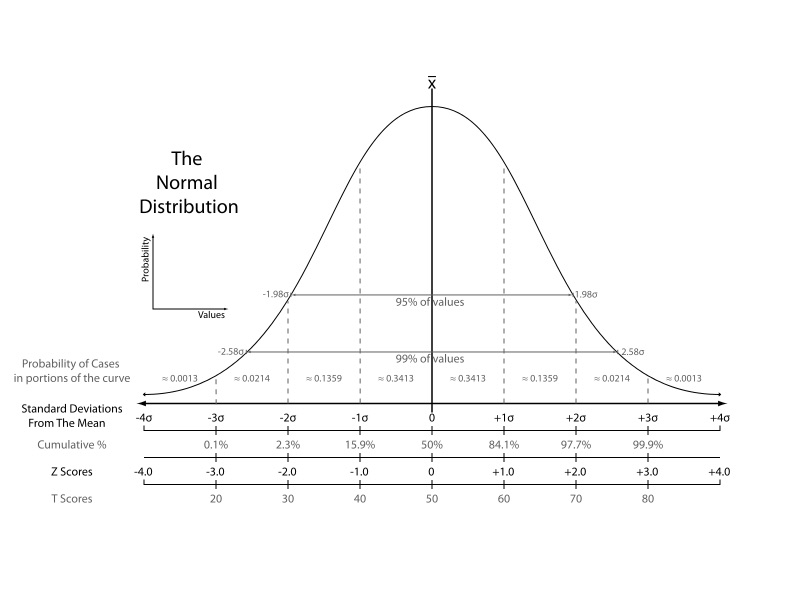
\includegraphics[width=\linewidth]{The_Normal_Distribution}
  \caption{More probability density is found as one gets closer to the expected (mean) value in a normal distribution. Statistics used in standardized testing assessment are shown. The scales include standard deviations, cumulative percentages, percentile equivalents, Z-scores, T-scores, standard nines, and percentages in standard nines..}
  \label{fig:marginfig}
\end{marginfigure}


\normalsize

\section{Introduction}
Statistics is the study of the collection, analysis, interpretation, presentation, and organization of data.[1] In applying statistics to, e.g., a scientific, industrial, or societal problem, it is conventional to begin with a statistical population or a statistical model process to be studied. Populations can be diverse topics such as "all persons living in a country" or "every atom composing a crystal". Statistics deals with all aspects of data including the planning of data collection in terms of the design of surveys and experiments.


%this generates 1cm of vertical space
\vspace{1cm}
\section{Statistics library}

\marginnote[30pt]{In the begin, I need type in "import random" to start this statistics code .}

\marginnote[30pt]{	The first code in statistics library is the explanation of the zero, it is a basic mode to calculate.}

\marginnote[30pt]{The second code is to define the sum of array, it will help user to calculate the sum when the array is longer than affordability.}

\marginnote[30pt]{The third code is to define the rand of array, this code is start more complex than before, we need the n, mini and maxi to finish the calculation}



\begin{shaded}
\begin{verbatim}
import random

def zeros(n):
a=[]
for i in range(n):
a=a+[0]
return a
def sum_array(a):
s=0
for i in range(len(a)):
s=s+a[i]
return s
def rand_array(n,mini,maxi):
a=[]
for i in range(n):
a=a+[random.uniform(mini,maxi)]
return a
def avg(a):
return sum_array(a)/len(a)
def var(a):
s=0
for i in range(len(a)):
s=s+[a[i]**2]
m=avg(a)
return (s/len(a)-m**2)
def maximum(a):
m=-math.inf
for i in range(len(a)):
if a[i]>m:
m=a[i]
return m
\end{verbatim}
\end{shaded}
\marginnote[-200pt]{The fourth code is to know the average of the array, we will use the sum of array devide by lenth of array to calculate this, and we already know how to type the sum of array, so it is not a no clue function. }
\marginnote[-50pt]{In the fifth code, the var is when you define a function parameter and it is a variable number of parameters of meaning, so we can use this code to figure out it very convenient. }

\marginnote[30pt]{The sixth code is to calculate the maximum.}
\marginnote[30pt]{The seventh code is the histogram, we need use the value of mini,maxi,bins and a.}

\marginnote[30pt]{The last two code is bargraph and main, be honest, those two code is relatively strange for me, but in the statistics library, it will be a good supporting code to reduce your time for anytime you need to use those code. }
\begin{shaded}
\begin{verbatim}
def histogram(mini,maxi,bins,a):
h=zeros(bins)
w=(maxi-mini)/bins
for i in range(len(a)):
for j in range(bins):
if a[i]>(mini+j*w) and a[i]<(mini+(j+1)*w):
h[j]=j[j]+1
return h
def bargraph(a):
win=graphWin("BarGraph",400,400)
win.SetCoords(-1,-1,len(a)+1,maximum(a)+1)
for i in range(len(a)):
rec=Rectangle(Point(i,0),Point(i+1,a[i]))
rec.draw(win)
def main():
gauss=[]
for i in range(100):
gauss=gauss+[sum_array(rand_array(10,0,1))]
bargraph(histogram(0,10,10,gauss))

\end{verbatim}
\end{shaded}





\chapter{Graphics Library}

The graphics library is a library for making easy graphical objects in python. It was written by John Zelle for use with his book Python Programming: An
Introduction to Computer Science. This chapter is going to discuss the topics we covered during class. To use the library you have to import it first. For an explanation on how to import libraries see the section of the book.

\section{Creating a basic window}
The graphics library works as a programm of it own. A window gets updated as long as it gets changed or is waiting for a new command.
To draw somthing on a window we first have to create a window. A creation follows this pattern:
\begin{fullwidth}
\begin{python}
Window = GraphWin(WindowName, Width, Height)
Window.setCoords(StartX,StartY,WidthPixel,HeightPixel)
\end{python}
\end{fullwidth}

\section{Drawing on windows}
Now that we know how to create a window we can start drawing on it. There are various objects we can draw on windows. Because the graphics library uses its own coordinates system we need to use it for creating objects.
\begin{python}
Point(2,4) #Creates a point at 2,4
\end{python}
To actually draw in windows we have to use the draw command. 
\begin{python}
Window = GraphWin(WindowName, Width, Height)
Window.setCoords(StartX,StartY,WidthPixel,HeightPixel)
Obj = OurObject
Obj.draw(Window)
\end{python}
In this example we are drawing Obj to our window.

\subsection{Rectangles}
In python rectangles are drawn from the down left point to the top right point.
\begin{python}
Rect = Rectangle(Point(X1,Y1),Point(X2,Y2))
\end{python}
This creates a rectangle calles Rect at the position X1 and Y1 with the width X2 and height Y2. 
After you have created your basic reactangle you can also color it.
\begin{fullwidth}
\begin{python}
Rect = Rectangle(Point(X1,Y1),Point(X2,Y2))
Rect.setFill(color_rgb(255,0,0)) #Set the color for the reactangle
\end{python}
\end{fullwidth}
\subsection{Circles}
Of course you can also add circles to your window. Circles are drawn from their middle point to the setting of the size of their diameter.
\begin{python}
C = Circle(Point(X,Y),Point(RX,RY))
\end{python}
The Point(X,Y) is defining the position of the circle. The Point(RX,RY) is defining the radius of the circle.

\subsection{Text labels}
On a window it is very important to be able to use text. Because of that the graphics library also comes with a text object for windows.
\begin{python}
T = Text(Point(X,Y),StringText)
\end{python}
The example is self explaining. But this text is nothing special. To make it cool we need to modifie it a bit.
\begin{fullwidth}
\begin{python}
Text.setFace(Font)
 #Availible Fonts are 'helvetica','arial','courier','times roman'
Text.setSize(Size) #Size of the text
Text.setStyle(Style)
 #Availible styles 'bold','normal','italic', 'bold italic'
Text.setTextColor(Color) # Use color_rgb(r,g,b) as a color
\end{python}
\end{fullwidth}

\newpage
\subsection{Other usefull methods}
There are some other usefull methods for the graphics library. Obj can be any object of the graphics library.
\begin{fullwidth}
\begin{python}
Obj.setFill(Color) #Sets the color
Obj.clone() #Creates a new object with the same properties as Obj.
Obj.move(X,Y) #Moves the object
color_rgb(r,g,b) #Makes a color for use with this library
Window.getMouse() #Stops the programm until you press on the screen
\end{python}
\end{fullwidth}

\subsection{Example code}
This is an example code of the graphics library.

\begin{marginfigure}[170pt]
  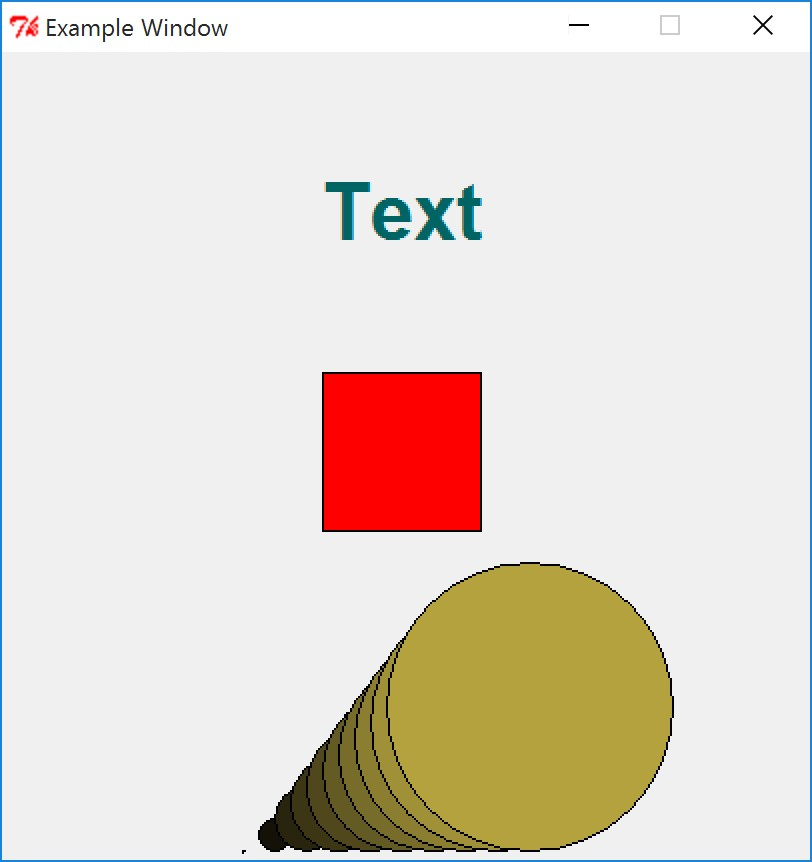
\includegraphics[width=\linewidth]{GraphicsExample1.jpg}
\end{marginfigure}
\begin{python}
from graphics import *

Win = GraphWin("Example Window",400,400)
Win.setCoords(0,0,50,50)
T = Text(Point(25,40), "Text")
T.draw(Win)
T.setFill(color_rgb(0,100,100))
T.setStyle("bold")
T.setFace("arial")
T.setSize(30)

Rect = Rectangle(Point(20,20),Point(30,30))
Rect.draw(Win)
Rect.setFill(color_rgb(255,0,0))

for i in range(10):
    C = Circle(Point(15+i*2,i),i)
    C.draw(Win)
    C.setFill(color_rgb(20*i,18*i,7*i))
\end{python}



















\chapter{Monte Carlo}
Monte Carlo simulations are a broad class of computational algorithms that rely on repeated random sampling to obtain numerical results. They are often used in physical and mathematical problems and are most useful when it is difficult or impossible to use other mathematical methods. Monte Carlo methods are mainly used in three distinct problem classes:[1] optimization, numerical integration, and generating draws from a probability distribution. In Class we have used the Monte Carlo simulation for the probability function.

We have estimated the value of pi 

    We start the familiar example of finding the area of a circle.  Figure 1 below shows a circle with radius r=1 inscribed within a square. The area of the circle is $Pi*r^2=Pi*1=Pi$ and the area of the square is 4 The ratio of the area of the circle to the area of the square is
    $[Graphics:Images/MonteCarloPiMod_gr_4.gif] $
    
        $[Graphics:Images/MonteCarloPiMod_gr_5.gif] $
        $[Graphics:Images/MonteCarloPiMod_gr_11.gif] $
\begin{verbatim} 
import random 
x=random.uniform(-1,1)
y=random.uniform(-1,1)
n=0.
#n is the number of random points in the circle
p=999999
#p is the number of random prints
for i in range(p):
    x=random.uniform(-1,1)
    y=random.uniform(-1,1)
    if (x*x+y*y)<1:
     n=n+1
pi=4*(n/p)
print pi
\end{verbatim}

As you increase P the estimation will be more accurate. for p=999999
\begin{verbatim}
>>> 
3.14152314152
>>> 
\end{verbatim}
Whereas for p=100
\begin{verbatim}
>>> 
3.24
>>> 
\end{verbatim}


\section {Game of Life}

The Game of Life, also known simply as Life, is a cellular automaton devised by the British mathematician John Horton Conway in 1970.
The "game" is a zero-player game, meaning that its evolution is determined by its initial state, requiring no further input. One interacts with the Game of Life by creating an initial configuration and observing how it evolves.
\subsection{ Game of Life Rules}
The universe of the Game of Life is an infinite two-dimensional orthogonal grid of square cells, each of which is in one of two possible states, alive or dead. Every cell interacts with its eight neighbours, which are the cells that are horizontally, vertically, or diagonally adjacent. At each step in time, the following transitions occur:
\begin{description}
  \item[First] \hfill \\
  Any live cell with fewer than two live neighbours dies, as if caused by under-population.
  \item[Second] \hfill \\
  Any live cell with two or three live neighbours lives on to the next generation.
  \item[Third] \hfill \\
  Any live cell with more than three live neighbours dies, as if by over-population.
  \item[Fourth] \hfill \\
  Any dead cell with exactly three live neighbours becomes a live cell, as if by reproduction.
  
\end{description}
 Here is the code we wrote in class: \hfill
\begin{verbatim}[frame=single]

import random
from graphics import *

#this function creates an NxN array filled with zeros
def empty(N):
    a=[]
    for i in range(N):
        b=[]
        for j in range(N):
            b=b+[0]
        a=a+[b]
    return a

#this function fills the array a with a portion p of live cells
def fill(a,p):
    N=len(a)
    for i in range(N):
        for j in range(N):
            if random.uniform(0,1)<p:
                a[i][j]=1

def update(A,B):
    N=len(A)
    for i in range(N):
        for j in range(N):
            neigh=A[(i-1)%N][(j-1)%N]+A[(i-1)%N][j]+A[(i-1)%N][(j+1)%N]+A[i][(j-1)%N]+A[i][(j+1)%N]+
            A[(i+1)%N][(j-1)%N]+A[(i+1)%N][j]+A[(i+1)%N][(j+1)%N]
            if A[i][j]==0:
                if neigh==3:
                    B[i][j]=1
                else:
                    B[i][j]=0
            else:
                if neigh==2 or neigh==3:
                    B[i][j]=1
                else:
                    B[i][j]=0


def gen2Dgraphic(N):
    a=[]
    for i in range(N):
        b=[]
        for j in range(N):
            b=b+[Circle(Point(i,j),.49)]
        a=a+[b]
    return a

def push(B,A):
    N=len(A)
    for i in range(N):
        for j in range(N):
            A[i][j]=B[i][j]
            
def drawArray(A,a,window):
#A is the array of 0,1 values representing the state of the game
#a is an array of Circle objects
#window is the GraphWin in which we will draw the circles
    N=len(A)
    for i in range(N):
        for j in range(N):
            if A[i][j]==1:
                a[i][j].undraw()
                a[i][j].draw(window)
            if A[i][j]==0:
                a[i][j].undraw()

N=10            #N is the number of live cells you start with
win = GraphWin("title",400,400)
win.setCoords(-1,-1,N+1,N+1)
grid=empty(N)
grid2=empty(N)
circles=gen2Dgraphic(N)
fill(grid,0.3)

while True:
    drawArray(grid,circles,win)
    update(grid,grid2)
    push(grid2,grid)
\end{verbatim}





\chapter{Git}
Git is a distributed revision control system with an emphasis on speed, data integrity, and support for distributed, non-linear workflows.  Git was initially designed and developed by Linus Torvalds for Linux kernel development in 2005, and has since become one of the most widely adopted version control systems for software development.

\begin{marginfigure}%
  
\includegraphics[width=\linewidth]{download.jpg}
  \label{fig:marginfig}
\end{marginfigure}
Please note the below assume you are using a Terminal shell in Linux or OSX operating system. If you are using Windows you will use "dir" instead of "ls" to list files using Command Terminal. Also note the slashes are different for writing file paths. Linux and OSX use forward slash / while Windows uses back slash.

\vspace{1cm}

\section{Introduce yourself to Git}

\begin{marginfigure}[60pt]

This is the first step you must do when using git for the first time. Tag your commits with Name and Email.
\end{marginfigure}
\begin{shaded}
\begin{verbatim}
$ git config --global user.name "Dr Doeg"
$ git config --global user.email doeg@example.com
\end{verbatim}
\end{shaded}


\newpage

\section{Basic Terminal Commands }

Using the terminal you may navigate the file directory.  Make, delete, move and rename files and directories.

\begin{margintable}[50pt]\index{unixfu}
  \footnotesize%
  \begin{center}
    \begin{tabular}{ll}
      \toprule
     Unix Command & Action \\
      \midrule
     \bf{cd}  & change directory        \\
    \bf{ls}  & list files        \\
     \bf{cp}  & list files        \\
      \bf{mv}  & move files        \\
       \bf{rm}  & remove files        \\
        \bf{rmdir}  & remove directory        \\
         \bf{touch}  & create file        \\
          \bf{nano}  & edit file        \\
           \bf{mkdir}  & create directory        \\
      \bottomrule
    \end{tabular}
  \end{center}
  \caption{A list of Unix shell commands.}
  \label{tab:font-sizes}
\end{margintable}


\begin{shaded}
\begin{verbatim}
$ cd path/to/project/folder
$ ls
$ cp filename ~/Location/newname
$ mv filename ~/Location/newname
$ rm filename
$ rmdir directoryname
$ touch filename
$ mkdir directoryname
$ nano filename
\end{verbatim}
\end{shaded}

\section{Git Repository}
You can get a Git project using two main approaches. The first takes an existing project or directory and imports it into Git. The second clones an existing Git repository from another server.

\section{Setting up a local Repository}
\marginnote[30pt]{Using the command line navigate to the project folder and initialize a git repository.}
\begin{shaded}
\begin{verbatim}
$ git init
\end{verbatim}
\end{shaded}
\marginnote[40pt]{Add files in the folder to the stage.\\ \ \\
\noindent Or add all the files.  }
\begin{shaded}
\begin{verbatim}
$ git add file2.jpg
$ git add .
\end{verbatim}
\end{shaded}
\marginnote[40pt]{Commit the additions.  }
\begin{shaded}
\begin{verbatim}
git commit -m "comment on the file changes"
\end{verbatim}
\end{shaded}

\newpage

\section{Push Your Local Repository to GitHub}

\marginnote[25pt]{\normalsize{Setup the remote repository location on GitHub using your account.}}
\begin{shaded}
\begin{verbatim}
$ git remote add origin https://github.com/<USER>/<REPO>.git
\end{verbatim}
\end{shaded}

\marginnote[40pt]{If you already set up the remote and want to change it use "set-url".}
\begin{shaded}
\begin{verbatim}
$ git remote set-url origin https://..../<USER>/<REPO>.git
\end{verbatim}
\end{shaded}
\marginnote[40pt]{Push the committed structure to the remote server.}
\begin{shaded}
\begin{verbatim}
$ git push origin master
\end{verbatim}
\end{shaded}

\vspace{1cm}

\section{Cloning an Existing Repository From GitHub }


\marginnote[40pt]{Navigate to the desired location in file structure.}
\begin{shaded}
\begin{verbatim}
$ cd path/to/whereUwant/folder
\end{verbatim}
\end{shaded}
\marginnote[40pt]{Set the location on the GitHub server to place the repositiory.}
\begin{shaded}
\begin{verbatim}
$ git clone https://github.com/<USER>/<REPO>.git
\end{verbatim}
\end{shaded}

\vspace{1cm}

\section{Working With Branches }
Version control is one of the great powers of git.

\begin{margintable}[80pt]\index{branchfu}
  \footnotesize%
  \begin{center}
    \begin{tabular}{ll}
      \toprule
     Unix Command & Action \\
      \midrule
     \bf{branch}  & list branches       \\
    \bf{branch} <NAME>  & create new branch        \\
    \bf{checkout} <NAME>  & switch to new branch        \\
     \bf{merge} <NAME>  & merge branch with current      \\
      \bf{branch -m} <NAME>  & rename current branch \\
      \bf{branch -D} <NAME>  & delete branch       \\
      \bottomrule
    \end{tabular}
  \end{center}
  \caption{A list of git commands for version control.}
  \label{tab:font-sizes}
\end{margintable}

\begin{shaded}
\begin{verbatim}
$ git branch
$ git branch branchname
$ git checkout branchname
$ git merge branchname
$ git branch -m newbranchname
$ git branch -D branchname
\end{verbatim}
\end{shaded}

\vspace{1cm}

\section{Updating an Existing Repository From GitHub }

\marginnote[20pt]{The sophisticated way to update uses fetch, reviews changes and merges those onto the master branch.  The alt the current project folder from the GitHub remote server.}
\begin{shaded}
\begin{verbatim}
$ git fetch
$ git pull -u origin master
\end{verbatim}
\end{shaded}

\vspace{1cm}

\section{Get Git, Github and More on Git}

\marginnote[10pt]{Download git and register an account at GitHub. Look at the official documentation for more information.}
https://git-scm.com/downloads  \\
\noindent https://github.com/  \\
\noindent  https://git-scm.com/book/en/v2










>>>>>>> upstream/master
%\include{rotational_kinematics}
%\include{forces}
%\include{work} 
%\include{momentum} 
%\include{angular_momentum} 





%\bibliography{sample-handout}
\bibliographystyle{plainnat}



\printindex

\end{document}


